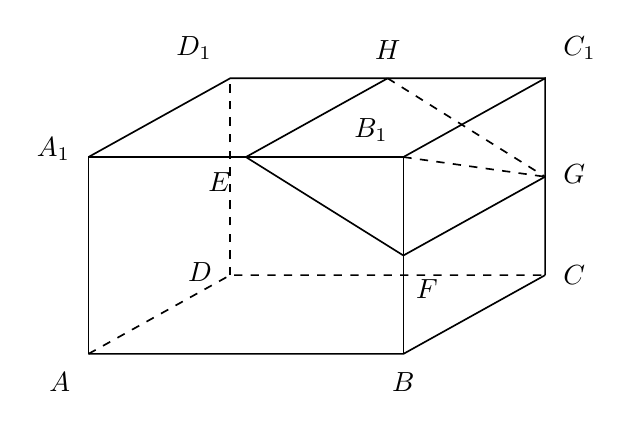
\begin{tikzpicture}[x=1cm,y=1cm,line width=0.6pt,font=\normalsize]
\coordinate (A) at (0,0);
\coordinate (B) at (4,0);
\coordinate (C) at (5.8,1);
\coordinate (D) at (1.8,1);
\coordinate (A1) at (0,2.5);
\coordinate (B1) at (4,2.5);
\coordinate (C1) at (5.8,3.5);
\coordinate (D1) at (1.8,3.5);
\coordinate (E) at (2.0000000000,2.5000000000);
\coordinate (H) at (3.8000000000,3.5000000000);
\coordinate (F) at (4.0000000000,1.2500000000);
\coordinate (G) at (5.8000000000,2.2500000000);
% visible cuboid
\draw[solid] (A)--(B)--(C);
\draw[solid] (A)--(A1)--(B1)--(B);
\draw[solid] (B1)--(C1)--(C);
\draw[solid] (A1)--(D1)--(C1);
% hidden cuboid
\draw[dashed] (A)--(D)--(C);
\draw[dashed] (D)--(D1);
\draw[dashed] (B1)--(G);
% section EFGH
\draw[solid] (E)--(H);
\draw[solid] (E)--(F);
\draw[solid] (F)--(G);
\draw[dashed] (H)--(G);
% labels with clearance
\node[below left,xshift=-3pt,yshift=-3pt] at (A) {$A$};
\node[below,yshift=-3pt] at (B) {$B$};
\node[right,xshift=3pt] at (C) {$C$};
\node[left,xshift=-3pt,yshift=1.0pt] at (D) {$D$};
\node[left,xshift=-3pt,yshift=3.0pt] at (A1) {$A_{1}$};
\node[above left=2pt] at (B1) {$B_{1}$};
\node[above right,xshift=3pt,yshift=3pt] at (C1) {$C_{1}$};
\node[above left,xshift=-3pt,yshift=3pt] at (D1) {$D_{1}$};
\node[below left=2pt] at (E) {$E$};
\node[below right=2pt,xshift=-1pt,yshift=-3pt] at (F) {$F$};
\node[right,xshift=3pt,yshift=1.0pt] at (G) {$G$};
\node[above,yshift=3pt] at (H) {$H$};
\end{tikzpicture}
